%\documentclass[iop]{emulateapj}
\documentclass[aps, pre, onecolumn, nofootinbib, notitlepage, groupedaddress, amsfonts, amssymb, amsmath, longbibliography]{revtex4-1}
\usepackage{tabularx}
\usepackage{graphicx}
\usepackage{hyperref}
\usepackage{xcolor}
\hypersetup{
    colorlinks,
    linkcolor={red!50!black},
    citecolor={blue!50!black},
    urlcolor={blue!80!black}
}
\usepackage{bm}
\usepackage{natbib}
\usepackage{longtable}
\LTcapwidth=0.87\textwidth

\newcommand{\Div}[1]{\ensuremath{\nabla\cdot\left( #1\right)}}
\newcommand{\DivU}{\ensuremath{\nabla\cdot\bm{u}}}
\newcommand{\angles}[1]{\ensuremath{\left\langle #1 \right\rangle}}
\newcommand{\grad}{\ensuremath{\nabla}}
\newcommand{\RB}{Rayleigh-B\'{e}nard }
\newcommand{\stressT}{\ensuremath{\bm{\bar{\bar{\Pi}}}}}
\newcommand{\lilstressT}{\ensuremath{\bm{\bar{\bar{\sigma}}}}}
\newcommand{\nrho}{\ensuremath{n_{\rho}}}
\newcommand{\approptoinn}[2]{\mathrel{\vcenter{
	\offinterlineskip\halign{\hfil$##$\cr
	#1\propto\cr\noalign{\kern2pt}#1\sim\cr\noalign{\kern-2pt}}}}}

\newcommand{\appropto}{\mathpalette\approptoinn\relax}

\newcommand\mnras{{MNRAS}}%

\begin{document}
\author{Evan H. Anders}
\affiliation{Dept. Astrophysical \& Planetary Sciences, University of Colorado -- Boulder, Boulder, CO 80309, USA}
\affiliation{Laboratory for Atmospheric and Space Physics, Boulder, CO 80303, USA}
\author{Benjamin P. Brown}
\affiliation{Dept. Astrophysical \& Planetary Sciences, University of Colorado -- Boulder, Boulder, CO 80309, USA}
\affiliation{Laboratory for Atmospheric and Space Physics, Boulder, CO 80303, USA}
\author{Jeffrey S. Oishi}
\affiliation{Department of Physics and Astronomy, Bates College, Lewiston, ME 04240, USA}
\title{Accelerated convergence of convective simulations using boundary value problems}

\begin{abstract}
We present a method for using coupling Boundary value problems (BVPs) with Initial value problems (IVPs)
in order to achieve thermally converged convective solutions on dynamical timescales, rather than the
long thermal timescale.  We demonstrate the similarity between the solution reached via BVP and the
solution reached by a long thermal rundown of the IVP, and demonstrate that this method works at a
large range of supercriticalities.  We use this method to achieve converged solutions at high Ra,
and discuss its extension to more complex scenarios, such as stratified, compressible convection.
\end{abstract}
\maketitle

\section{To Do}
\begin{enumerate}
\item Get 3D cases in
\item Run some fixed T boundary conditions to see that we get the scaling expected from 
\cite{johnston&doering2009}.  Literally re-do their experiment.
\item Continue Improving Figures
\item Write figure captions
\item Think about creating a 2-roll vs. 3-roll figure to help explain that part
\item Think about post-bvp multiplying.  Should it be a profile for both the velocity
and for the T perturbations, rather than a scalar?  I'm starting to think it should.
\end{enumerate}


\section{Introduction}
\label{sec:intro}
Natural convection occurs in the presence of disparate timescales. Granules on the
solar surface overturn on the order of 10 minutes, whereas deep motions in the Sun are likely at
low Mach number and constrained by the solar rotation rate of $\sim$1 month.  
Despite these relatively short dynamical times, the scale of energy transport on the
Sun occurs on the Kelvin-Helmholtz timescale of nearly $3 \times 10^7$ \emph{years} \cite{stix2003}. 
As simulations aim to model natural convection
by increasing into the high-Rayleigh Number (Ra) regime, where diffusive timescales are much
longer than dynamical timescales \cite{Anders&Brown2017}, achieving converged simulations will 
require runs which span a greater number of convective timescales in order to thermally converge.
Furthermore, with increasing Ra and decreasing diffusivities, motions become more turbulent
and require finer grid meshes and smaller timesteps to resolve turbulent motions, meaning that
achieving even one overturn timescale becomes a harder problem.  
These two effects combine such that achieving thermally converged, high-Ra, astrophysically interesting
simulations is intractable using modern numerical tools.

In studies of stratified convection where a convective layer lies between stable layers, studies
have used the knowledge of Mixing Length Theory (MLT) to adjust the initial thermal profile of
atmospheres to a state which is closer to the adiabat chosen by convection \cite{brandenburg&all2005}.
However, many studies of convection do not contain stable layers above and below the convection
zone, and the presence of hard boundaries and the boundary layers that they form makes it difficult to
know proper evolved adiabat \emph{a priori} before the dynamics of the simulation evolve the
structure of the boundary layers.

Here we present a method for using simple boundary value problems (BVPs), 
along with information about the evolved flow fields,
to fast-forward the slow thermal evolution of convecting simulations.  
We run two sets of experiments: one in which we allow convective simulations to evolve for a
full thermal timescale before taking measurements, and another in which we employ a fast-forwarding,
BVP technique which occurs on dynamical timescales. We compare these two sets of simulations to
show the validity of the BVP technique.  Then, we use the BVP technique to run simulations
at high Ra, in the regime where running for thermal timescales becomes computationally intractable.

\section{Experiment}
\label{sec:experiment}
In our study, we adopt the Oberbeck-Boussinesq approximation.  Here, the
fluid has constant kinematic viscosity ($\nu$), thermal diffusivity ($\kappa$), and coefficient
of thermal expansion ($\alpha$).  We non-dimensionalize length by the layer height ($L_z$) ,
temperature by the (constant) initial temperature gradient across the layer ($\grad T_0$), and time
by the freefall timescale ($L_z / v_{\text{ff}}$, with $v_{\text{ff}} = \sqrt{\alpha g L_z^2 \grad T_0}$, where $g$ is 
uniform gravitational acceleration in the $-\hat{z}$ direction). The dimensionless Boussinesq
equations governing the velocity $\bm{u} = u\hat{x} + v\hat{y} + w\hat{z}$, temperature
$T = T_0 + T_1$, and reduced pressure $\varpi$ are \cite{spiegel&veronis1960}
\begin{gather}
\DivU = 0, 
	\label{eqn:incompressible}
\\
\frac{\partial \bm{u}}{\partial t} + \bm{u}\cdot\grad\bm{u} =
-\grad\varpi + T_1\hat{z} + \frac{\text{Pr}}{\text{Ra}}\grad^2\bm{u}, 
	\label{eqn:bouss_momentum}
\\
\frac{\partial T_1}{\partial t} + \bm{u}\cdot\grad(T_0 + T_1) = \frac{1}{\text{Pr}\,\text{Ra}}\grad^2 T_1,
	\label{eqn:bouss_energy}
\end{gather}
where the dimensionless control parameters are the Rayleigh and Prandtl numbers,
\begin{equation}
\text{Ra} = \frac{g \alpha L_z^4 \grad T_0}{\nu\chi} = \frac{(L_z\,v_{\text{ff}})^2}{\nu\chi}, \qquad \text{Pr} = \frac{\nu}{\chi}.
\end{equation}
The dimensionless vertical extent of the domain is $z = [-1/2, 1/2]$, and at the boundaries
we impose no-slip, impenetrable boundary conditions such that $w = u = v = 0$ at $z = \pm 1/2$.
At the lower boundary, we employ a fixed flux condition such that $\partial T_1 / \partial z = 0$
at $z = -1/2$, and we impose a fixed temperature condition $T_1 = 0$ at $z = 1/2$. Both
horizontal directions are periodic, extending over a range $x, y = [0, \Gamma]$, where
the aspect ratio is $\Gamma = 2 \lambda_c$, with
$\lambda_c = 2\pi/k_c$, and $k_c=2.5519$ is the wavenumber of convective onset for this choice of
boundary conditions.  

The chosen thermal boundary conditions at the upper and lower plates
determine key quantities of the evolved state.
Studies of incompressible, Boussinesq, \RB convection often
employ fixed temperature (Dirichlet) or fixed heat flux
(Neumann) boundary conditions at both plates.  
Dirichlet conditions represent plates of infinite conductivity,
whereas Neumann conditions model plates of finite conductivity.  
In both cases, choosing symmetric boundary conditions maintains overall system symmetry, 
and despite evolving towards different thermal structures, both types of conditions
transport heat in the same manner \cite{johnston&doering2009}.
Studies of convection which aim to model
astrophysical systems such as stars often employ a mixture of these
two types of boundary conditions \cite{hurlburt&all1984, cattaneo&all1991, korre&all2017}.  
The flux at the lower boundary is fixed, modeling
the constant energy generation of the stellar core, 
while the outer boundary condition is held at a fixed temperature,
modeling the surface of a star which must output the energy generated internally.
This setup is a useful model for understanding natural
systems, but simulations which employ these boundary conditions suffer from a long 
thermal relaxation as the atmosphere loses energy and approaches the adiabat chosen by the
Dirichlet condition.  We choose these conditions in part to better understand them, and in
part because these conditions minimize the number of assumptions that must be made in
setting up the boundary value problem.




\subsection{The Boundary Value Problem}
\begin{figure}[b]
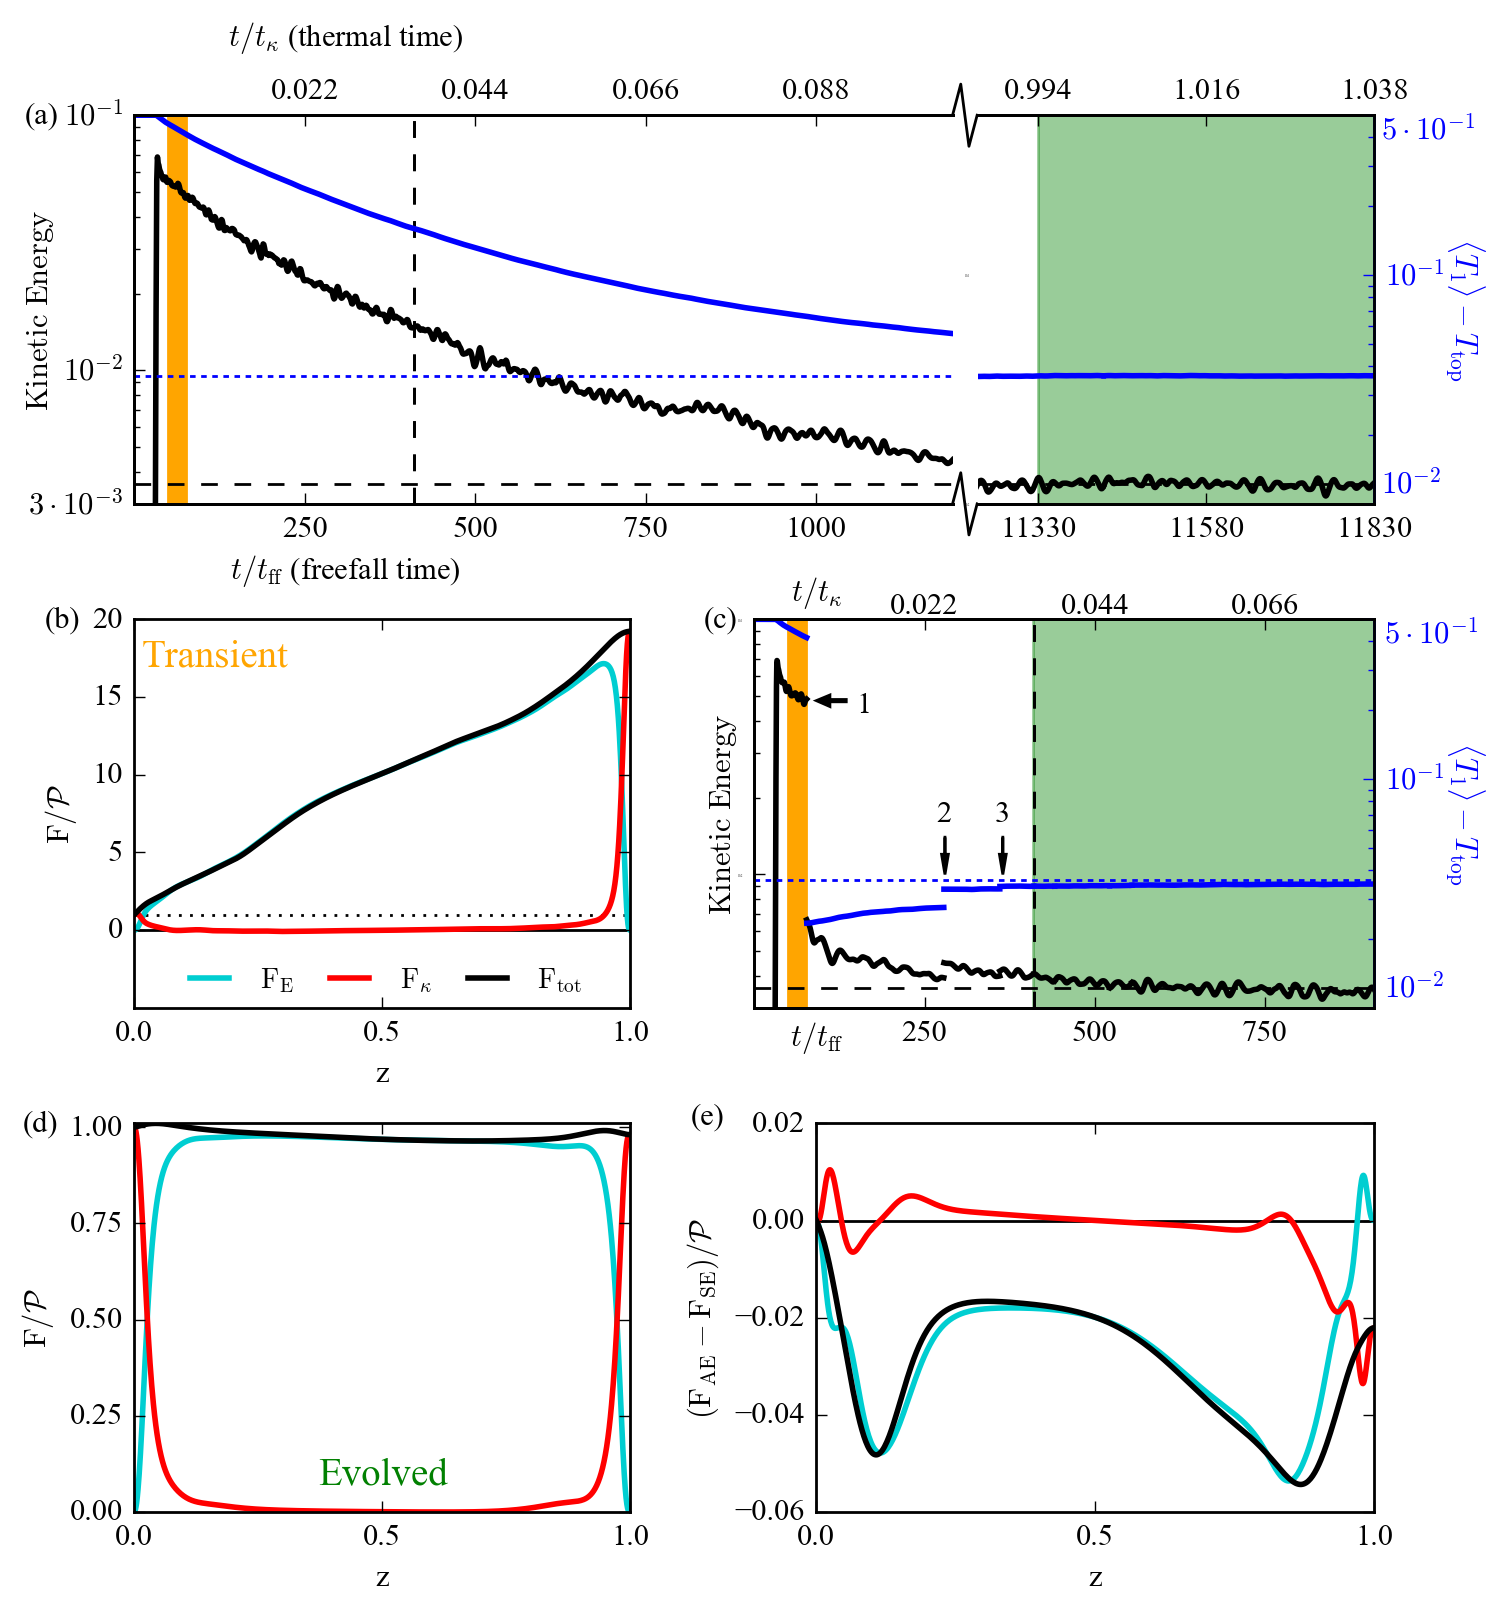
\includegraphics[width=\textwidth]{./figs/time_trace.png}
\caption{\label{fig:time_trace} }
\end{figure}

The prohibitively long thermal timescale required to reach an equilibrium temperature profile
in a Direct Numerical Simulation (DNS) can be skipped by coupling the DNS with a simple Boundary Value Problem
(BVP) solve. Using information about the dynamics of the convection in the atmosphere, it is possible
to skip a large portion of the thermal evolution, see Fig \ref{fig:time_trace}a\&b.

The Boussinesq BVP contains equations of hydrostatic balance and thermal equilibrium,
\begin{gather}
\frac{\partial}{\partial z}\angles{\varpi} = \angles{T_1}\hat{z},
	\label{eqn:bouss_BVP_momentum}
\\
\frac{\partial}{\partial z}\angles{wT_1} = \frac{1}{\text{Pr}\text{Ra}}\frac{\partial^2}{\partial z^2} \angles{T_1},
	\label{eqn:bouss_BVP_energy}
\end{gather}
where $\angles{A}$ represents a time- and horizontally averaged profile of the quantity $A$.  
These
equations arise from taking time- and horizontal- averages of Eqns (\ref{eqn:bouss_momentum}\&\ref{eqn:bouss_energy}),
neglecting terms that vanish due to symmetry, and assuming that the flows are in a stationary state.  
Convective flows
are perturbations around a thermal profile defined by these equations in the proper evolved state.

Under eqns (\ref{eqn:bouss_BVP_momentum}\&\ref{eqn:bouss_BVP_energy}), 
the thermal structure ($\angles{T_1}$, $\angles{\varpi}$) of the atmosphere is fully determined by the specification
of the convective flux, $F_{conv} = \angles{w T_1}$.  If this profile is known, then 
solving for $\angles{T_1}$ and
$\angles{\varpi}$ depends only upon the choice of boundary conditions.

By definition, the profile of $F_{conv}$ is \emph{not} in its time stationary state near the
beginning of the simulation.  In fact, under mixed boundary conditions, as the atmosphere approaches the
isotherm specified by the upper boundary condition, the motions display an asymmetric flux as energy
leaks through the upper boundary condition (Fig. \ref{fig:time_trace}c).  
In order to construct the evolved convective flux from the current fluxes in the atmosphere,
we acknowledge that the evolved solution will be in flux equilibrium, 
carrying the amount of flux specified at the fixed-flux condition throughout the full depth of the atmosphere.  
Thus, the steady-state profile of the convective flux can be approximated as
\begin{equation}
F_{\text{conv, steady}} = F_{\text{bot}}\frac{\angles{wT_1}}{\angles{wT_1 - \kappa \partial_z (T_0 + T_1)}}
= F_{\text{bot}}\frac{\angles{F_{\text{conv, IVP}}}}{\angles{F_{\text{tot, IVP}}}}.
\label{eqn:bouss_BVP_fconv}
\end{equation}
In essence, the construction of this profile assumes that the system appropriately picks out the ratios
\begin{equation}
f_{\text{conv}} = \frac{F_{\text{conv}}}{F_{\text{tot}}}\qquad
f_{\text{cond}} = \frac{F_{\text{cond}}}{F_{\text{tot}}}.
\end{equation}
in the transient state.  Thus, even though the quantity of flux being carried is not correct, the
system is carrying flux convectively where it needs to in the interior, and conductively in the boundaries.

The choice of a fixed-flux boundary condition at the bottom appropriately scales the magnitude of
$F_{\text{conv, steady}}$.  The choice of a fixed-temperature boundary condition at the top of the
atmosphere appropriately sets the isotherm of the convective interior.  While this method can be used
for other choices of thermal boundary conditions (see Discussion), dual fixed temperature conditions
at the upper plate require a more careful handling of $F_{\text{bot}}$, and dual fixed flux boundary
conditions have degenerate solutions for the constant offset of $T_1$.

In general, the BVP solve takes the following form:
\begin{enumerate}
\item Run the convective IVP. Once the convection begins, start taking averages averages of $\angles{wT_1}$
and $\partial_z^2\angles{T_1}$, which determine the fluxes through the system.  Update these averages every
$\Delta t = 0.1$ freefall times.  Once these averages are converged to 1 part in 1000, the BVP is ready to be solved.
\item Construct $F_{\text{conv, steady}}$ from the flux profiles, then use it to solve for $\angles{T_1}$ 
and \angles{\varpi} of the
evolved state.  Adjust the mean profiles in the BVP such that this is their mean profile.
\item Divide the velocities and the $T_1$ fluctuations around the mean profile by 
$\sqrt{\bar{F_{\text{bot}}/F_{\text{tot}}}}$. This lowers the convective flux through the system such that it is,
on average, the convective flux used in the BVP solve.
\item Continue running the IVP for a number of freefall times to allow the velocities and temperature perturbations
to equilibrate to the new mean state.
\end{enumerate}
This procedure seems to work quite well, see Fig. \ref{fig:time_trace}d\&e.


\subsection{Numerics}
We utilize the 
Dedalus\footnote{\url{http://dedalus-project.org/}} 
pseudospectral framework \cite{burns&all2016} to time-evolve  
(\ref{eqn:incompressible})-(\ref{eqn:bouss_energy}) 
using an implicit-explicit (IMEX), third-order, four-step 
Runge-Kutta timestepping scheme RK443 \cite{ascher&all1997}.  
The temperature field is decomposed as $T = T_0(z) + T_1(x, y, z, t)$
and the velocity is $\bm{u} = w\bm{\hat{z}} + u\bm{\hat{x}} + v\bm{\hat{y}}$.
In our 2D runs, $v = 0$.
Variables are time-evolved on a dealiased Chebyshev (vertical)
and Fourier (horizontal, periodic) domain in which the
physical grid dimensions are 3/2 the size of the coefficient grid.  
Domain sizes range from
32x128 coefficients at the lowest values of 
Ra to 1024x4096 coefficients at Ra $> 10^{9}$ in 2D.

As initial conditions, we fill $T_1$ with
random white noise whose magnitude is $10^{-6}(\text{Ra Pr})^{-1/2}$.
This ensures that the initial perturbations are much smaller than the
evolved convective temperature perturbations, even at large Ra.
We filter this noise spectrum in coefficient space, 
such that only the lower 25\% of the coefficients
have power.

In 2D, there are often multiple steady state solutions (e.g., 2-roll and 3-roll
solutions) which have slightly different flow properties (heat transport, etc.).
Even though the initial perturbations are very small, they shape the convective
transient and thus determine the nature of the steady state convection, at least in
the laminar regime.  In order to ensure that our results are not biased by differences
in flow structure, we ran the simulations using distinct random temperature perturbations
so as to compare statistics in comparable flow fields.  In 3D, rolls are nonstationary over
convective timescales, and so these effects need not be considered there.

\section{Results}
While the differences in the fluxes in Fig. \ref{fig:time_trace} are small, it is important
to determine if the velocity fluctuations and point-by-point nonlinear transport are the same
in the evolved state.  Fig. \ref{fig:pdf_comparison} overlays the probability distribution functions
of the vertical and horizontal velocities, as well as the fully nonlinear portion of the convective
flux for the same case as is shown in Fig. \ref{fig:time_trace}.  The PDFs are quite similar visually,
and have a similarity of (XYZ) according to a Kolmogorov-Smirnov statistic.

In addition to getting the nonlinear dynamics mostly correct, we show that the BVP method retrieves the
proper temperature profile, see e.g., Fig. \ref{fig:temp_comparison}.  Here the BVP profile retrieves the
mean profile of the temperature to within 1\% accuracy, and temperature fluctuations in the two runs
have a similarity of (XYZ) according to a Kolmogorov-Smirnov statistic.

This method works across a broad range of supercriticality.  In Fig. \ref{fig:parameter_space_comparison},
we show measurements of the volume-averaged Nusselt number, Reynolds number, and temperature.
We use standard definitions of the Nusselt number and Reynolds numbers,
\begin{equation}
\text{Nu} = \frac{\angles{wT - (\text{Ra Pr})^{-1/2}\grad T}}{\angles{- (\text{Ra Pr})^{-1/2} \grad T}} =
1 + \frac{\angles{wT}}{-\Delta T}\sqrt{\text{Ra Pr}}, \qquad \text{Re} = \frac{|\bm{u}| L_z}{\nu},
\end{equation}
where $\Delta T = T(z = 1/2) - T(z = -1/2)$ is the evolved temperature difference
between the top and bottom plates.  This form of the Nusselt number is valid even when
the system is not yet in flux equilibrium, and reduces to the standard fixed flux definition
of Nu  = $[1 - \angles{wT} / P]^{-1}$ \cite{johnston&doering2009}. We find a scaling law of
Nu $\propto \text{Ra}^{2/3}$, much steeper than a standard 2/7 or 1/3 scaling law
\cite{johnston&doering2009}. Furthermore, we find that Re$\propto \text{Ra}^{0.425}$. The average temperature
approaches the value at the top of the domain as Ra increases.  

The final morphology of the flows is very important in determining the exact value of Nu and Re.  In general,
a two-roll state vs. a three-roll state will have entirely different statistics -- different Nu, Re, and average
temprature (and as a result, different size boundary layers).  Thus, in 2D studies, it is essential to study flows
of a similar morphology in order to see a clear trend. 

\begin{figure}[t]
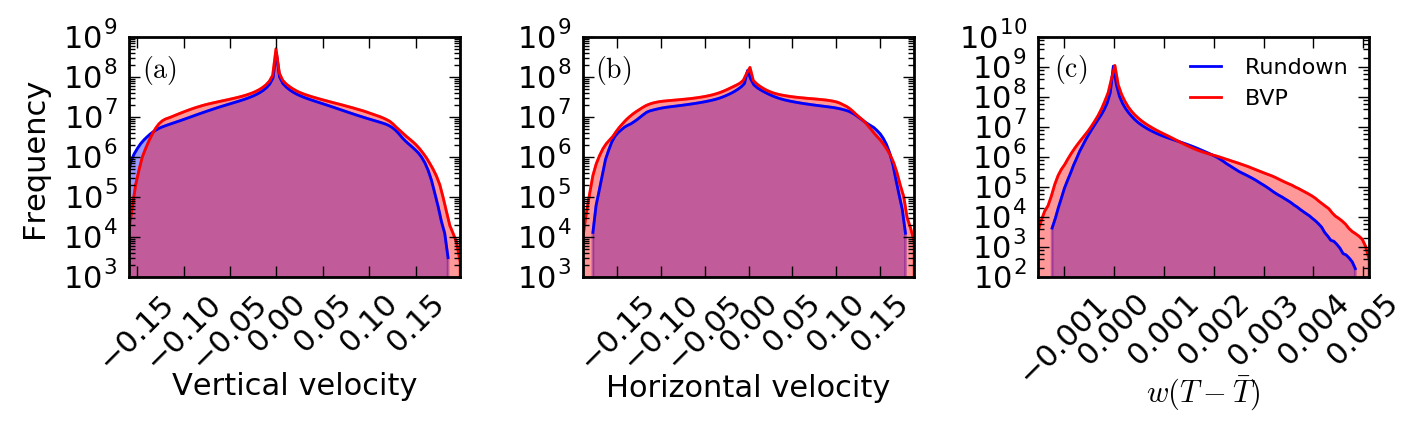
\includegraphics[width=\textwidth]{./figs/pdf_comparison.png}
\caption{\label{fig:pdf_comparison} }
\end{figure}

\begin{figure}[t]
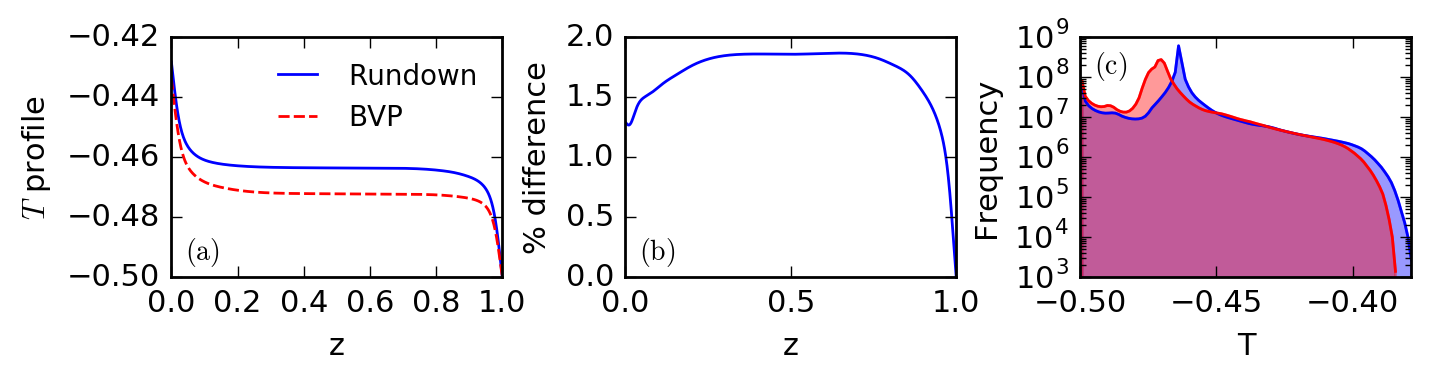
\includegraphics[width=\textwidth]{./figs/temp_comparison.png}
\caption{\label{fig:temp_comparison} }
\end{figure}

\begin{figure}[t]
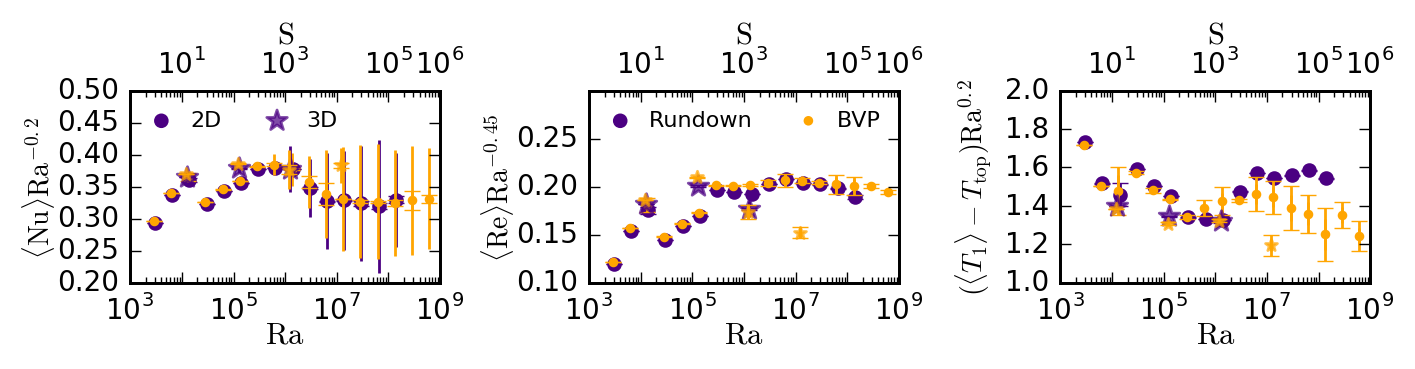
\includegraphics[width=\textwidth]{./figs/parameter_space_comparison.png}
\caption{\label{fig:parameter_space_comparison} }
\end{figure}



\section{Discussion \& Conclusions}
\label{sec:results}
I don't have the mental stamina to write this section right now.  In general, here's what it's going to say:
\begin{enumerate}
\item This procedure works, as we've shown.
\item How to apply this to more complicated cases, like stratified convection
\item How to apply this to different boundary conditions
\item Brief discussion of other methods that can be used to fast-forward, e.g., bootstrapping.
\item This is just a first step.
\end{enumerate}




\begin{acknowledgments}
EHA acknowledges the support of the University of Colorado's George 
Ellery Hale Graduate Student Fellowship.
This work was additionally supported by  NASA LWS grant number NNX16AC92G.  
Computations were conducted 
with support by the NASA High End Computing (HEC) Program through the NASA 
Advanced Supercomputing (NAS) Division at Ames Research Center on Pleiades
with allocations GID s1647 and GID g26133.
\end{acknowledgments}


\appendix
\section{Table of Runs}
\begin{center}
\begin{tabularx}{\textwidth}{ X X X X X X X }
\hline													
Ra	&	Supercriticality	&	nz	&	nx	&	$t_{\text{therm}}$	&	$t_{\text{post BVP}}$	&	$t_{\text{avg}}$	\\[1ex]
\hline		\hline											
$2.79 \cdot 10^3$	&	$10^{1/3}$	&	32	&	128	&	$52.8$	&	50	&	100	\\
$6.01 \cdot 10^3$	&	$10^{2/3}$	&	32	&	128	&	$77.6$	&	50	&	100	\\
$1.30 \cdot 10^4$	&	$10^1$	&	32	&	128	&	$114$	&	50	&	100	\\
$2.79 \cdot 10^4$	&	$10^{1 + 1/3}$	&	32	&	128	&	$167$	&	50	&	100	\\
$6.01 \cdot 10^4$	&	$10^{1 + 2/3}$	&	32	&	128	&	$245$	&	50	&	100	\\
$1.30 \cdot 10^5$	&	$10^2$	&	64	&	256	&	$360$	&	100	&	100	\\
$2.79 \cdot 10^5$	&	$10^{2 + 1/3}$	&	64	&	256	&	$528$	&	100	&	100	\\
$6.01 \cdot 10^5$	&	$10^{2 + 2/3}$	&	64	&	256	&	$776$	&	100	&	100	\\
$1.30 \cdot 10^6$	&	$10^3$	&	128	&	512	&	$1.14 \cdot 10^3$	&	100	&	200	\\
$2.79 \cdot 10^6$	&	$10^{3 + 1/3}$	&	128	&	512	&	$1.67 \cdot 10^3$	&	200	&	200	\\
$6.01 \cdot 10^6$	&	$10^{3 + 2/3}$	&	256	&	1024	&	$2.45 \cdot 10^3$	&	200	&	200	\\
$1.30 \cdot 10^7$	&	$10^4$	&	256	&	1024	&	$3.60 \cdot 10^3$	&	200	&	200	\\
$2.79 \cdot 10^7$	&	$10^{4 + 1/3}$	&	256	&	1024	&	$5.28 \cdot 10^3$	&	200	&	200	\\
$6.01 \cdot 10^7$	&	$10^{4 + 2/3}$	&	256	&	1024	&	$7.76 \cdot 10^3$	&	200	&	200	\\
$1.30 \cdot 10^8$	&	$10^5$	&	512	&	2048	&	$1.14 \cdot 10^4$	&	500	&	500	\\
$2.79 \cdot 10^8$	&	$10^{5 + 1/3}$	&	512	&	2048	&	$1.67 \cdot 10^4$	&	500	&	500	\\
$6.01 \cdot 10^8$	&	$10^{5 + 2/3}$	&	512	&	2048	&	$2.45 \cdot 10^4$	&	500	&	500	\\
$1.30 \cdot 10^9$	&	$10^6$	&	1024	&	4096	&	$3.60 \cdot 10^4$	&	500	&	500	\\
\hline													
\end{tabularx}
\end{center}



\bibliography{biblio.bib}
\end{document}
